\documentclass[sigconf]{webmedia}

\usepackage{listings}
\usepackage{hyperref}
\usepackage{caption}
\usepackage{subcaption}
\usepackage{tikz}
\usetikzlibrary{arrows.meta, calc, positioning, shapes.geometric}

\graphicspath{{assets/}}

\newcommand{\projectname}{\texttt{gingaf}}
\newcommand{\CCWS}{CCWS}

%% \BibTeX command to typeset the BibTeX logo in the docs
\AtBeginDocument{%
  \providecommand\BibTeX{{%
    \normalfont B\kern-0.499em{\scshape i\kern-0.25em b}\kern-0.8em\TeX}}}

\settopmatter{printacmref=false, printfolios=false}

%% Choose the appropriate event.
\setevent{webmedia}
\proceedingsDetails[WebMedia’2026]{Proceedings of the Brazilian Symposium on Multimedia and the Web}{2026}{Lavras/MG, Brazil} 
\ISSN{2966-2753}

\begin{document}

\title{\projectname{}: A Cross-Platform Architecture to Execute Ginga-NCL and Ginga-HTML5 Applications}

\author{Alan L. V. Guedes}
\orcid{0000-0003-0110-9975}
\email{a.guedes@reading.ac.uk}
\affiliation{%
  \institution{University of Reading}
  \country{UK}
}

\author{Paulo Victor Borges}
\orcid{0009-0002-3620-477X}
\email{paulo.victor.lima15@gmail.com}
\affiliation{%
  \institution{PUC-Rio}
  \country{Brazil}
}

\author{Daniel Moraes}
\orcid{0000-0003-2995-3115}
\email{danielmoraes@telemidia.puc-rio.br}
\affiliation{%
  \institution{PUC-Rio}
  \country{Brazil}
}

\author{Sergio Colcher}
\orcid{0000-0002-3476-8718}
\email{colcher@puc-rio.br}
\affiliation{%
  \institution{PUC-Rio}
  \country{Brazil}
}

\renewcommand{\shortauthors}{Guedes et al.}

\begin{abstract}
Ginga, alongside its Ginga-NCL and Ginga-HTML5 subsystems, is an international standard for interactive digital television defined by the ITU-T/SBTVD. It is used in Brazil and several Latin American countries, and reaches over 60 million people. However, traditional Ginga development tools rely on heavy, platform-specific C++ implementations, creating a steep barrier to entry for developers. This paper presents \projectname{}, a Ginga architecture which focuses on decoupling  logic components from UI components to support running both Ginga-NCL and Ginga-HTML5 applications directly from the web browser, mobile, or desktop. On the web, we present a portable Lua interpreter and a Ginga-HTML5 player that intercepts HTTP requests to support Ginga-CC-WebServices. This architecture does not require any native browser plugins, paving the way for web-based development playgrounds and debugging environments.
\end{abstract}

\keywords{TV, Ginga, Ginga-NCL, Ginga-HTML5}

\begin{teaserfigure}
  \centering
  \begin{subfigure}{0.499\linewidth}
    \centering
    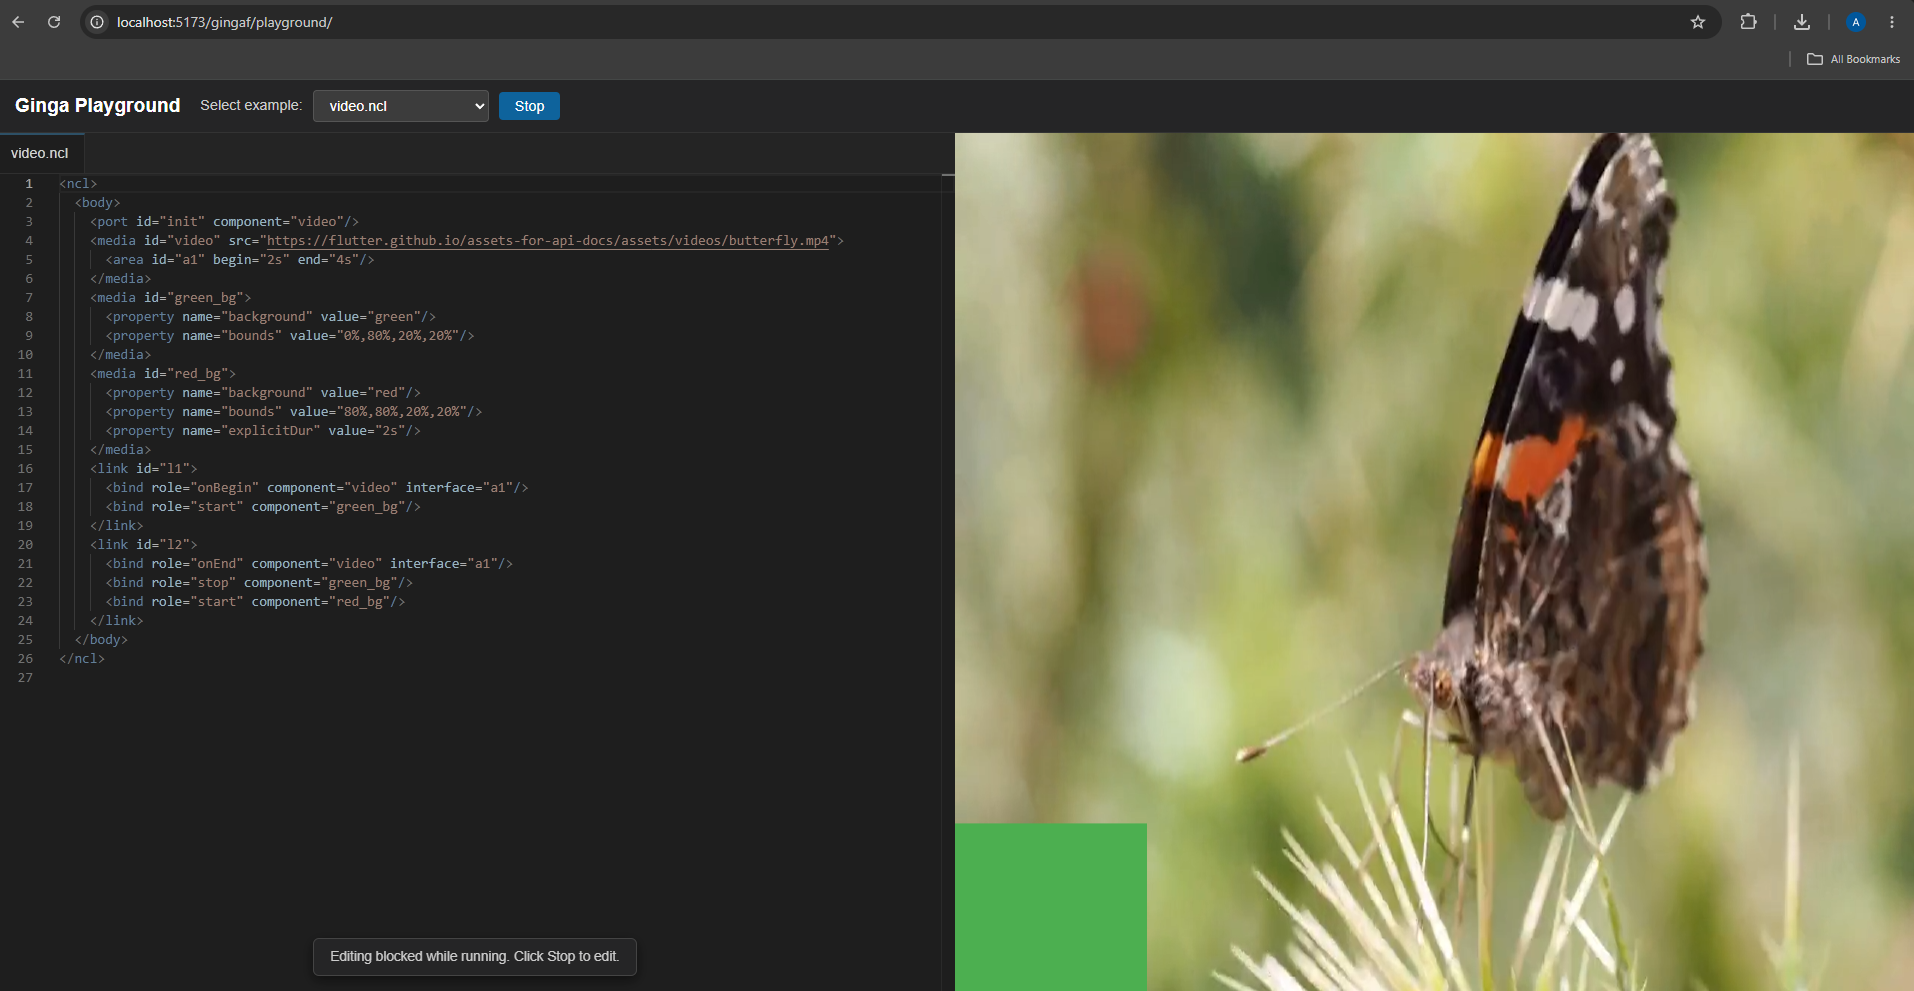
\includegraphics[width=\linewidth]{playground.png}
    \Description{Ginga-NCL application video.ncl executing a video at 2 seconds in the GingaPlayground interface.}
    \caption{Execution of Ginga-NCL application \texttt{video.ncl} at $t=2$s.}
    \label{fig:play1}
  \end{subfigure}%
  \hfill%
  \begin{subfigure}{0.499\linewidth}
    \centering
    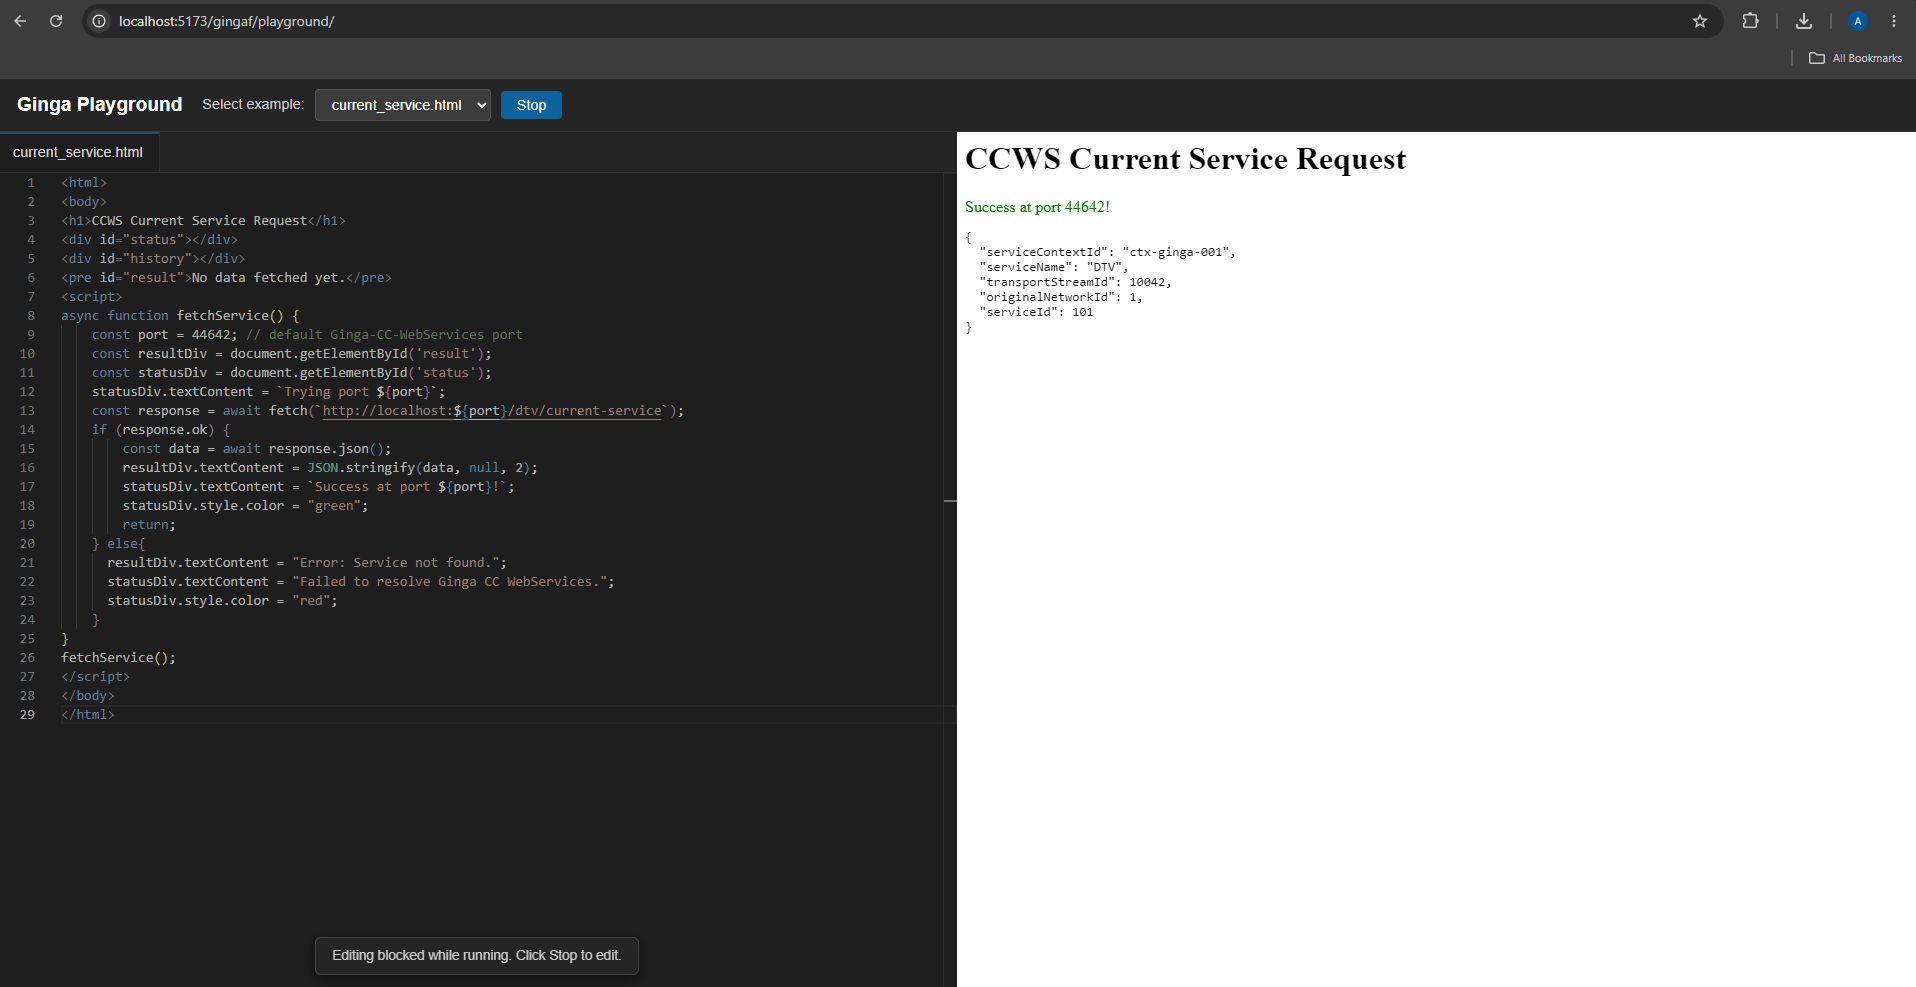
\includegraphics[width=\linewidth]{playground-html.png}
    \Description{Execution of a Ginga-HTML5 application current_service.html in the GingaPlayground interface.}
    \caption{Execution of Ginga-HTML5 application \texttt{current\_service.html}.}
    \label{fig:play2}
  \end{subfigure}\\[0.499em]
  \begin{subfigure}{0.499\linewidth}
    \centering
    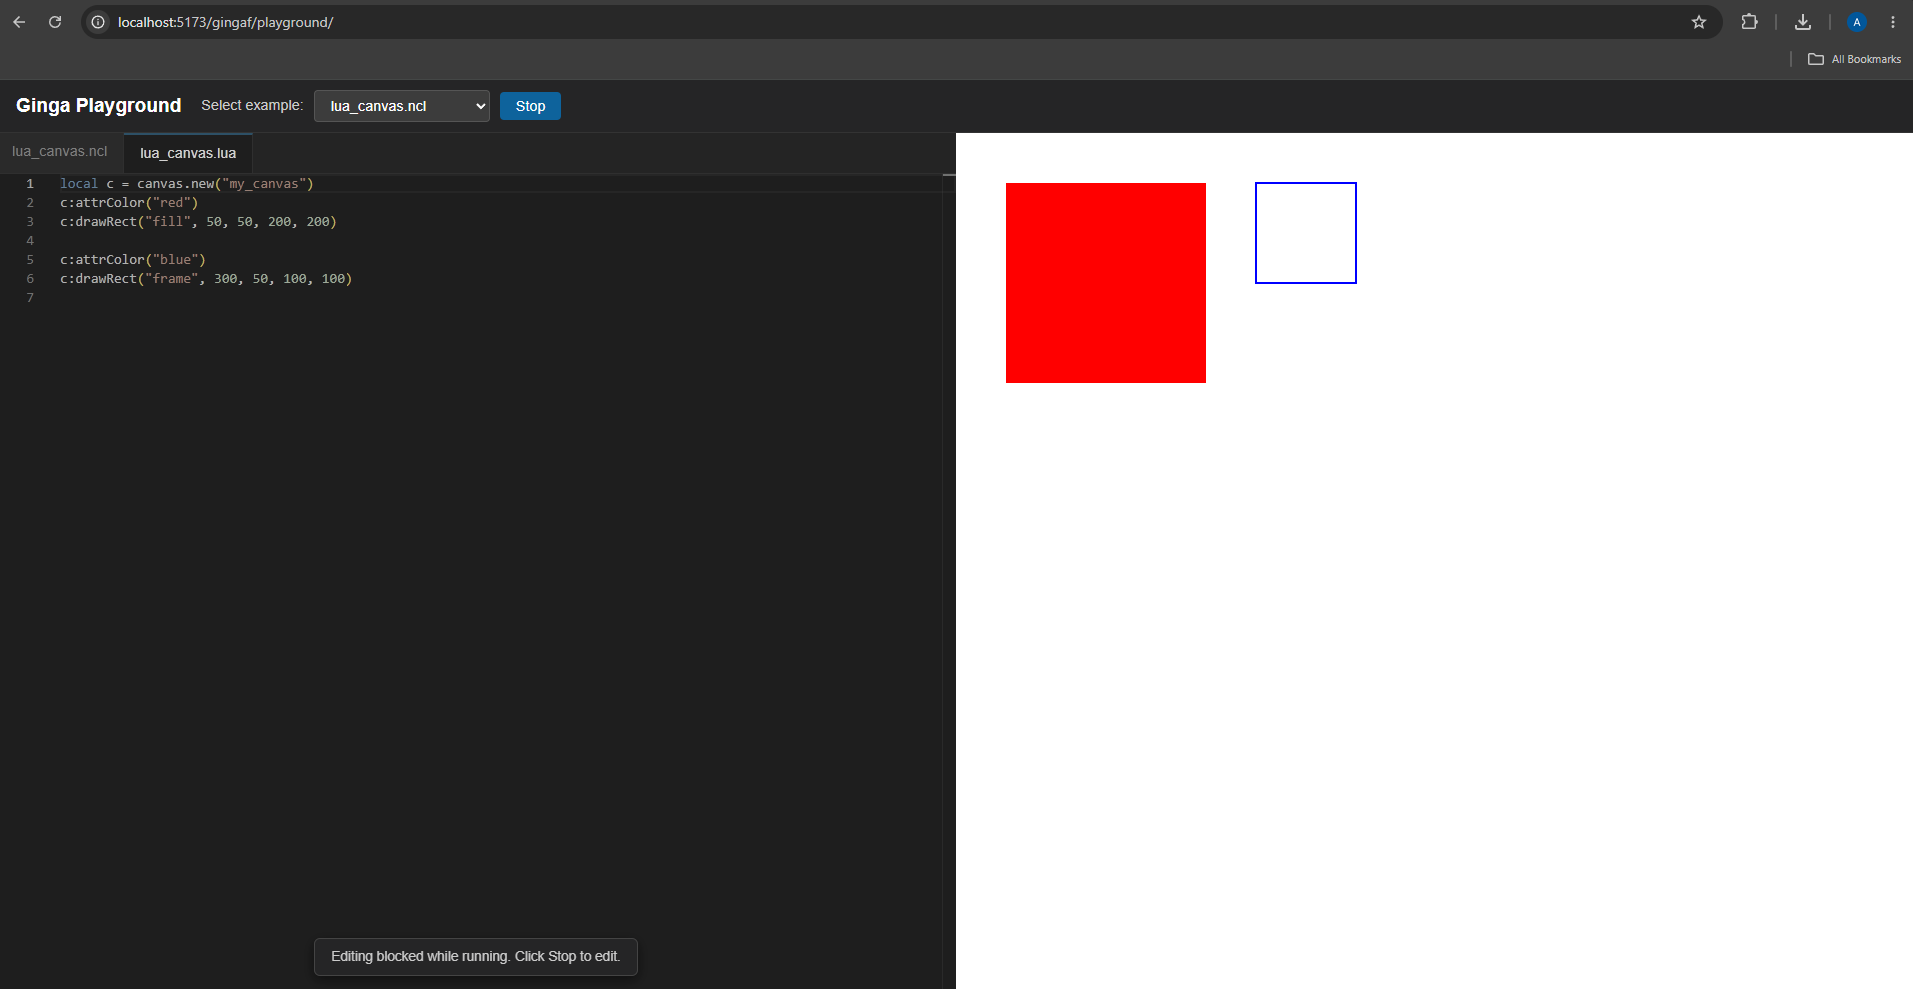
\includegraphics[width=\linewidth]{playground-lua.png}
    \Description{Execution of a Ginga-NCL application lua_canvas.ncl drawing shapes on canvas using Lua scripts in the GingaPlayground interface.}
    \caption{Execution of Ginga-NCL application \texttt{lua\_canvas.ncl}}
    \label{fig:play3}
  \end{subfigure}
  \caption{\projectname{} execution at Web using the GingaPlayground interface}
  \label{fig:playground_res}
\end{teaserfigure}

\maketitle

\section{Introduction}

The Ginga middleware is the international standard for interactive digital television by both the ITU-T~\cite{ITU_H761} and the Brazilian Digital Terrestrial Television System (SBTVD)~\cite{abnt_15606_2_2023}. Ginga utilizes the Nested Context Language (NCL), an XML-based declarative multimedia language. Ginga standard is legally mandated and installed on 100\% of certified Digital TV sets and set-top boxes sold in Brazil and several other Latin American countries adopting the ISDB-T framework. Because it is mandated by local telecommunications entities, every major television manufacturer must embed a Ginga implementation directly into their hardware firmware, making it one of the most widely deployed interactive middleware systems globally. This wide adoption results in over 60 million people impacted daily. It is also widely used for public interest broadcasting; for example, the Brazil4D~\cite{castro2016brazil} application targets low-income families to access public services, health information, and educational content. Furthermore, the application coding specification for the next-generation Brazilian digital television standard (TV 3.0) continues to advance the Ginga engine~\cite{santos2026overview}. 

Despite the critical role and massive scale of Ginga, developers and researchers continue to face the \textbf{lack of a Web-based development environment}. This happens because traditional Ginga players, such as the reference PUC-Rio C++ implementations~\cite{ginga2013, ginga2018}, are tightly coupled to the native platform (targeting Linux-based digital TV receivers) and require specialized OS setups, compilers, and heavy multimedia frameworks to run. Moreover, the recent standardisation of new Ginga subsystems (Ginga-HTML5 and Ginga-CC-WebServices) added more complexity and limited the portability of these traditional C++ players. Therefore, developers and researchers cannot easily share, test, or prototype their code online. This creates a steep barrier, which contrasts sharply with the trend in modern programming ecosystems, where major frameworks provide instant web-based playgrounds. 

\projectname{} addresses these challenges by introducing a portable Ginga architecture that focuses on decoupling logic and UI components.  By separating the logic (headless) execution engine from the visual rendering layer, we support running both subsystems directly from the web browser, mobile, or desktop. As a proof of concept and validation of this decoupled design, we developed GingaPlayground (Figure~\ref{fig:playground_res}), a web-based editor running directly in the browser without any native plugins or local installation.

To support reproducibility, source code (both \projectname{} and GingaPlayground), unit tests, and demonstration videos of \projectname{} are available\footnote{\url{https://github.com/ginga-org-br/gingaf}}. An instance of GingaPlayground is hosted online\footnote{\url{https://ginga-org-br.github.io/gingaf/playground/}}.

We summarize our main contributions below:

\begin{itemize}
  \item \textbf{Cross-Platform Ginga implementation by Decoupling Logic from UI Components}: We introduce an architecture that strictly separates the headless logic state from the presentation components. This decoupling enables deterministic execution of Ginga synchronization logic in pure code environments and cross-platform support across web, mobile, and desktop from a single codebase.
  \item \textbf{NCLua and CCWS Support on the Web}: We present adaptations for embedding NCLua and CCWS to be able to run client-side by using a portable pure Dart Lua interpreter and overloading the browser's \texttt{fetch} API inside a sandboxed iframe.
\end{itemize}



The remainder of this paper is structured as follows. Section~\ref{sec:background} presents the background on the Ginga standard, and Section~\ref{sec:relatedwork} reviews related work. Section~\ref{sec:methodology} introduces the decoupled architecture of \projectname{}. Section~\ref{sec:nclplayer} and Section~\ref{sec:htmlccws} detail the execution of the Ginga-NCL and Ginga-HTML5 subsystems. Section~\ref{sec:playground} presents the GingaPlayground use case. Finally, Section~\ref{sec:remarks} concludes the paper.

\section{Ginga Background}
\label{sec:background}

Figure~\ref{fig:architecture} depicts the architecture of the D-profile Ginga DTV Receiver introduced by the TV 2.5 specifications~\cite{moreno2020brief}. Dashed elements are the new components proposed in D-profile receivers, namely, Ginga-HTML5 and Ginga-CC-WebServices. In the following, we first detail the main components\footnote{Other components such as SI and DSMCC were omitted for simplicity.}.

\begin{figure}[!ht]
    \centering
    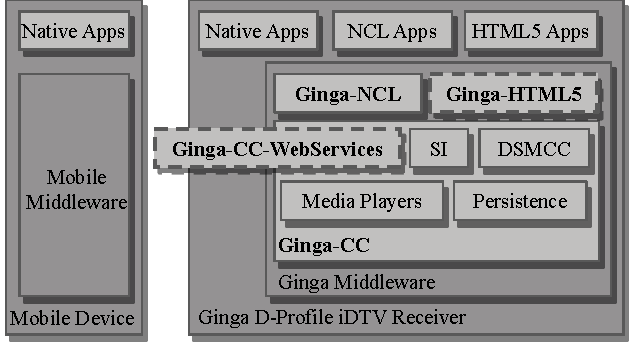
\includegraphics[width=\linewidth]{ginga.pdf}
    \Description{Decoupled architecture of the D-Profile Ginga Receiver, showing the separated headless logic and rendering components for Ginga-NCL, NCLua, Ginga-HTML5, and Ginga-CC-WebServices.}
    \caption{D-Profile Ginga Receiver (Source: \cite{moreno2020brief}).}
    \label{fig:architecture}
\end{figure}

\textbf{Ginga-NCL} is the subsystem responsible for controlling NCL multimedia applications. NCL~\cite{soares_nested_2006_model} is a declarative language that defines temporal synchronization, layout reuse, multi-device presentation, and embedded Lua scripting\footnote{\url{https://www.lua.org}}. It also provides an API for on-the-fly modifications (NCL editing commands) and handles media from both broadcast and broadband channels. To accommodate varying hardware capabilities, the SBTVD Forum defines specific receiver profiles that applications can target to ensure compatibility~\cite{abnt_15606_2_2023}.


To demonstrate the structure of NCL applications, we use a sample application (\texttt{video.ncl}) presented in Listing~\ref{lst:ncl}. The presentation defines a primary video (\texttt{video}) in lines~\ref{line:video_start}--\ref{line:video_end}, a green background media (\texttt{green\_bg}) in lines~\ref{line:green_start}--\ref{line:green_end}, and a red background media (\texttt{red\_bg}) in lines~\ref{line:red_start}--\ref{line:red_end} with an explicit duration of 2 seconds. Temporal behavior is coordinated by link elements: link \texttt{l1} starts the green background when area \texttt{a1} of the video begins (at 2s), and link \texttt{l2} stops the green background and starts the red background when area \texttt{a1} ends (at 4s). The application ends when the \texttt{red\_bg} ends at 6s (explicitDur 2s) and the main video ends decoding at 7s (video content duration). 

\newpage


\begin{lstlisting}[language=XML, escapeinside={(*}{*)}, caption={video.ncl source code}, basicstyle=\scriptsize\ttfamily, frame=single, breaklines=true, aboveskip=1mm, belowskip=1mm, captionpos=b, numbers=left, label={lst:ncl}]
<ncl>
<body>
  <port id="init" component="video"/>
  <media id="video" src="https://flutter.github.io/assets-for-api-docs/assets/videos/butterfly.mp4">(*\label{line:video_start}*)
    <area id="a1" begin="2s" end="4s"/>
  </media>(*\label{line:video_end}*)
  <media id="green_bg">(*\label{line:green_start}*)
    <property name="background" value="green"/>
    <property name="bounds" value="0%,80%,20%,20%"/>
  </media>(*\label{line:green_end}*)
  <media id="red_bg">(*\label{line:red_start}*)
    <property name="background" value="red"/>
    <property name="bounds" value="80%,80%,20%,20%"/>
    <property name="explicitDur" value="2s"/>
  </media>(*\label{line:red_end}*)
  <link id="l1">
    <bind role="onBegin" component="video" interface="a1"/>
    <bind role="start" component="green_bg"/>
  </link>
  <link id="l2">
    <bind role="onEnd" component="video" interface="a1"/>
    <bind role="stop" component="green_bg"/>
    <bind role="start" component="red_bg"/>
  </link>
</body>
</ncl>
\end{lstlisting}

\textbf{Ginga-HTML5}~\cite{abnt_15606_10_2026} supports the execution of Web-based applications (\textit{e.g.}, Listing~\ref{lst:html5}) natively within the Ginga environment. It provides a standard web engine capable of rendering HTML5, CSS3, and executing JavaScript, allowing developers to author interactive digital television applications using modern web technologies. 

\textbf{Ginga-CC-WebServices} focuses on integrating the experience of the broadcasting and broadband environments.
To do this, it supports a set of services implemented in the form of REST APIs.
Thus, as indicated in Figure~\ref{fig:architecture}, its functionalities can be used by:
1) native Smart TV applications, web-based applications, and Ginga applications in the DTV receiver;
2) devices present in the home environment, allowing, \textit{e.g.}, second-screen scenarios. 

According to its standard~\cite{abnt_15606_11}, Ginga-CC-WebServices listens by default on port 44642 and can be discovered by multicasting an HTTP M-SEARCH request.
Its functionalities include not only functions for accessing content from broadcasting, but also functions that standardize access to advanced features of the DTV environment (\textit{e.g.},  platform characteristics, supported DRM, media playback capabilities). 
We briefly introduce each API and show its main endpoints in what follows.
In particular, the identifiers in square brackets should be filled in the API request. For instance, the \texttt{GET} \texttt{http(s)://\textless{}host\textgreater{}/dtv/current-service} returns information for the selected DTV service.

To demonstrate the structure of Ginga-HTML5 applications using Ginga-CC-WebServices, we provide a sample application in Listing~\ref{lst:html5}. This JavaScript-based HTML application uses the standard \texttt{fetch} API to request the \texttt{/dtv/current-service} endpoint on the local Ginga-CC-WebServices server at the default port 44642. Once the asynchronous request is resolved, the application parses the JSON response and updates the \texttt{div} elements with the retrieved service data or an error message if the service is unreachable.

\newpage

\begin{lstlisting}[language=HTML, caption={\texttt{current\_service.html} fetching from Ginga-CC-WebServices}, basicstyle=\scriptsize\ttfamily, frame=single, breaklines=true, aboveskip=1mm, belowskip=1mm, captionpos=b, numbers=left, label={lst:html5}]
<html>
<body>
<h1>Ginga-CC-WebServices Current Service Request</h1>
<div id="status"></div>
<div id="history"></div>
<pre id="result">No data fetched yet.</pre>
<script>
async function fetchService() {
    const port = 44642; // default Ginga-CC-WebServices port
    const resultDiv = document.getElementById('result');
    const statusDiv = document.getElementById('status');
    statusDiv.textContent = `Trying port ${port}`;
    const response = await fetch(`http://localhost:${port}/dtv/current-service`);
    if (response.ok) {
        const data = await response.json();
        resultDiv.textContent = JSON.stringify(data, null, 2);
        statusDiv.textContent = `Success at port ${port}!`;
        statusDiv.style.color = "green";
        return;
    } else{
      resultDiv.textContent = "Error: Service not found.";
      statusDiv.textContent = "Failed to resolve Ginga-CC-WebServices.";
      statusDiv.style.color = "red";
    }
}
fetchService();
</script>
</body>
</html>
\end{lstlisting}



\section{Related Work}
\label{sec:relatedwork}

The development of Ginga players has historically been led by the TeleMídia Lab at PUC-Rio, producing several versions. However, all prior implementations share a fundamental limitation: they are deeply tethered to native desktop libraries, making web compilation impossible. Earlier work such as WebNCL~\cite{webncl2013} provided a web-based NCL presentation engine but did not support Lua scripting.
\begin{table*}[!ht]
  \centering
  \caption{Comparison of NCL Player Implementations}
  \label{tab:comparison}
  \resizebox{\linewidth}{!}{%
    \begin{tabular}{l c c c c c c c c}
      \toprule
      \textbf{Work} & \textbf{Language} & \textbf{Multimedia Engine} &  \textbf{Web Deploy} & \textbf{Mobile Deploy} & \textbf{Scheduling} & \textbf{Ginga-NCL} & \textbf{Ginga-HTML5} & \textbf{CCWS} \\
      \midrule
       PUC-Rio Ginga v0.13 \cite{ginga2013,moreno2010conciliando} & C++ & SDL/FFmpeg & No & No & Event-Listener & Yes & No & No \\
       PUC-Rio Ginga v1.0~\cite{ginga2018,dodsworth2018dynamic} & C++ & GTK/Gstreamer & No & No & Synchronous \texttt{tick()} & Yes & No & No \\
      WebNCL~\cite{webncl2013} & JavaScript & HTML5 &Yes & No & Event-Listener & Yes & No & No \\
      NuGinga~\cite{nuginga18,nuginga_playcode20} & C++ (WASM) & HTML5 & Yes & Yes & Event-Listener & Yes & No & No \\
      \projectname{} (ours) & Dart & Flutter & Yes & Yes & Synchronous \texttt{tick()} & Yes & Yes & Yes \\
      \bottomrule
    \end{tabular}%
  }
\end{table*}

\begin{figure}[h!]
  \centering
  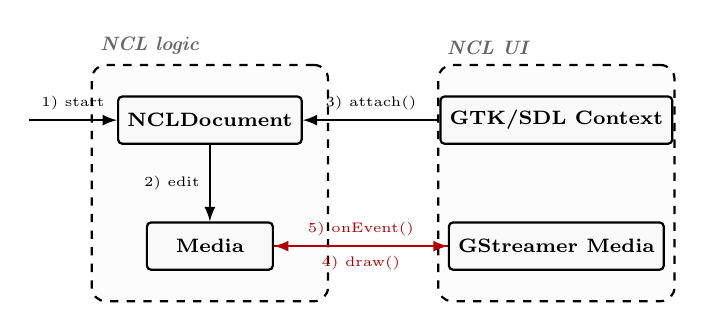
\begin{tikzpicture}[
    package/.style={draw, rectangle, rounded corners=5pt, minimum width=3.0cm, minimum height=3.0cm, fill=gray!2, dashed, thick, align=center},
    comp/.style={draw, rectangle, rounded corners=1.5pt, minimum width=1.6cm, minimum height=0.6cm, fill=gray!5, thick, align=center, font=\scriptsize},
    arrow/.style={-latex, thick},
    redarrow/.style={-latex, thick, color=red!70!black}
  ]
    \node[package] (doc_pkg) at (0, 0) {};
    \node[anchor=south west, font=\scriptsize\bfseries\itshape, text=gray!80!black] at (doc_pkg.north west) {NCL logic};

    \node[package] (app_pkg) at (4.4, 0) {};
    \node[anchor=south west, font=\scriptsize\bfseries\itshape, text=gray!80!black] at (app_pkg.north west) {NCL UI};

    \node[comp] (doc) at (0, 0.8) {\textbf{NCLDocument}};
    \node[comp] (media) at (0, -0.8) {\textbf{Media}};
    \node[comp] (ui) at (4.4, 0.8) {\textbf{GTK/SDL Context}};
    \node[comp] (ui_media) at (4.4, -0.8) {\textbf{GStreamer Media}};

    \draw[arrow] (-2.3, 0.8) -- (doc.west) node[midway, above, font=\tiny] {1) start};
    \draw[arrow] (doc) -- (media) node[midway, left, font=\tiny] {2) edit};
    \draw[arrow] (ui) -- (doc) node[midway, above, font=\tiny] {3) attach()};
    \draw[redarrow] (media) -- (ui_media) node[midway, below, font=\tiny] {4) draw()};
    \draw[redarrow] (ui_media) -- (media) node[midway, above, font=\tiny] {5) onEvent()};
  \end{tikzpicture}
  \Description{Traditional native C++ NCL player architecture describing PUC-Rio Ginga v0.13 and v1.0, demonstrating tight coupling between logic elements and UI graphics bindings.}
  \caption{Traditional native C++ NCL player architecture describing PUC-Rio Ginga v0.13 and v1.0, demonstrating tight coupling between logic elements and UI graphics bindings.}
  \label{fig:old_arch}
\end{figure}

PUC-Rio Ginga v0.13.6~\cite{ginga2013,moreno2010conciliando} was designed for early-generation digital TV receivers with resource constraints. It used SDL\footnote{\url{https://www.libsdl.org}} as the UI context for rendering graphics and managing window events, and FFmpeg\footnote{\url{https://ffmpeg.org}} for audio/video decoding. Its execution model relied on event listeners to handle asynchronous media playback: dedicated threads monitored AV decoder callbacks and posted events into the NCL engine, creating concurrency that was difficult to test deterministically. Recently, PUC-Rio Ginga v1.0~\cite{ginga2018,dodsworth2018dynamic} modernized the renderer by adopting GTK\footnote{\url{https://www.gtk.org}} as the UI context and GStreamer\footnote{\url{https://gstreamer.freedesktop.org}} as the AV decoding pipeline. A key architectural advance was the move to a mono-threaded model inspired by synchronous execution: rather than spawning per-media threads, the engine advances state through a central tick loop, reducing race conditions and improving predictability. Another notable early implementation is \textbf{WebNCL}, a web-based NCL player fully implemented in JavaScript that did not support Lua.

The fundamental architectural issue preventing these implementations from running on the web is the tight coupling between the NCL logic layer and the native operating system resources. As illustrated in Figure~\ref{fig:old_arch}, in traditional C++ Ginga architectures, a \texttt{Media} object within the NCL Document directly instantiates and drives a native multimedia element (such as a GTK widget or a GStreamer pipeline). The state machine logic blocks on native rendering calls (\texttt{draw()}), and the media objects trigger NCL transitions directly via system thread callbacks (\texttt{onEvent()}). 

This bidirectional, tightly bound architecture makes it exceptionally difficult to virtualize the execution. In a web browser environment (\textit{e.g.}, using WebAssembly), there is no access to raw socket connections for Ginga-CC-WebServices, no native threading model compatible with GStreamer, and no direct frame buffer for GTK to paint onto. Furthermore, JavaScript's single-threaded event loop and strict security sandboxes make blocking NCL state machine evaluations completely incompatible with web execution.

Recent efforts to modernize NCL tooling have explored cross-platform frameworks. One crucial related work is NuGinga Playcode~\cite{nuginga_playcode20}, a web-compatible NCL authoring tool supporting NCL and NCLua using cross-compilation techniques. This work demonstrated the feasibility of porting NCL and Lua to the web by using C++ to Wasm toolchains. Our work, \projectname{}, extends this capability by providing a fully decoupled Dart implementation that natively supports both HTML (via Ginga-CC-WebServices integration) and Lua without heavily relying on C++ to Wasm toolchains.

Table~\ref{tab:comparison} compares the features of \projectname{} with traditional implementations. By completely decoupling the logic component from the UI component, and by porting the logic entirely to pure Dart, \projectname{} successfully isolates the synchronization engine. This allows the logic to compile flawlessly to JavaScript and Wasm, completely sidestepping the historical native binding limitations.

\section{Methodology}
\label{sec:methodology}

To overcome the inherent coupling between NCL logic and native rendering pipelines, \projectname{} introduces a novel architecture built using Dart and the Flutter\footnote{\url{https://docs.flutter.dev/}} framework. A key architectural decision in our proposed architecture is the strict separation of the NCL state machine from the visual presentation layer, leveraging Dart's multiplatform capabilities. By implementing the core \texttt{NCLDocument} engine entirely in pure Dart as a non-UI component, we guarantee that the complex NCL logic can be natively compiled and executed across web, mobile, and desktop environments without requiring platform-specific bindings or C++ bridges. Figure~\ref{fig:layered_arch} illustrates this high-level layered architecture. 



\begin{figure}[ht!]
  \centering
  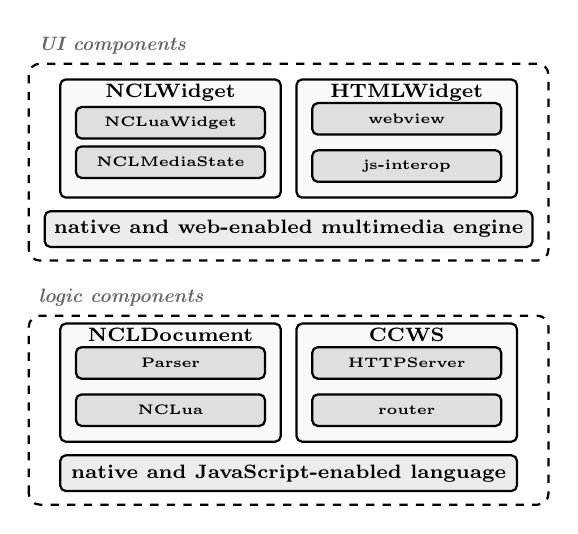
\begin{tikzpicture}[
    layer/.style={draw, rectangle, rounded corners=2pt, minimum height=0.4cm, fill=gray!15, thick, align=center, font=\scriptsize\bfseries},
    outerbox/.style={draw, rectangle, rounded corners=2pt, minimum height=1.5cm, fill=gray!5, thick, align=center, font=\scriptsize\bfseries},
    innerbox/.style={draw, rectangle, rounded corners=2pt, minimum height=0.4cm, fill=gray!25, thick, align=center, font=\tiny\bfseries},
    singlebox/.style={draw, rectangle, rounded corners=2pt, minimum height=1.5cm, fill=gray!5, thick, align=center, font=\scriptsize\bfseries},
    gingafbox/.style={draw, rectangle, rounded corners=4pt, dashed, thick, fill=none}
  ]
    \draw[gingafbox] (-3.3, 0.2) rectangle (3.3, 2.6);
    \node[anchor=south west, font=\scriptsize\bfseries\itshape, text=gray!80!black] at (-3.3, 2.6) {logic components};

    \draw[gingafbox] (-3.3, 3.3) rectangle (3.3, 5.8);
    \node[anchor=south west, font=\scriptsize\bfseries\itshape, text=gray!80!black] at (-3.3, 5.8) {UI components};

    \node[layer, minimum width=5.8cm] (dart) at (0, 0.6) {native and JavaScript-enabled language};
    
    \node[outerbox, minimum width=2.8cm] (ncldoc) at (-1.5, 1.75) {};
    \node[anchor=north, font=\scriptsize\bfseries, inner sep=2pt] at (ncldoc.north) {NCLDocument};
    \node[innerbox, minimum width=2.4cm] (parser_logic) at (-1.5, 2.0) {Parser};
    \node[innerbox, minimum width=2.4cm] (nclua_logic) at (-1.5, 1.4) {NCLua};
    
    \node[outerbox, minimum width=2.8cm] (ccws) at (1.5, 1.75) {};
    \node[anchor=north, font=\scriptsize\bfseries, inner sep=2pt] at (ccws.north) {CCWS};
    \node[innerbox, minimum width=2.4cm] (httpserver_logic) at (1.5, 2.0) {HTTPServer};
    \node[innerbox, minimum width=2.4cm] (router_logic) at (1.5, 1.4) {router};

    \node[layer, minimum width=5.8cm] (flutter) at (0, 3.7) {native and web-enabled multimedia engine};

    \node[outerbox, minimum width=2.8cm] (nclwidget) at (-1.5, 4.85) {};
    \node[anchor=north, font=\scriptsize\bfseries, inner sep=2pt] at (nclwidget.north) {NCLWidget};
    \node[innerbox, minimum width=2.4cm] (ncluawidget) at (-1.5, 5.05) {NCLuaWidget};
    \node[innerbox, minimum width=2.4cm] (nclmediastate_widget) at (-1.5, 4.55) {NCLMediaState};
    
    \node[outerbox, minimum width=2.8cm] (htmlwidget) at (1.5, 4.85) {};
    \node[anchor=north, font=\scriptsize\bfseries, inner sep=2pt] at (htmlwidget.north) {HTMLWidget};
    \node[innerbox, minimum width=2.4cm] (webview) at (1.5, 5.1) {webview};
    \node[innerbox, minimum width=2.4cm] (js_interop) at (1.5, 4.5) {js-interop};
  \end{tikzpicture}
  \Description{Layered architecture diagram of gingaf showing the separation between logic and UI components.}
  \caption{\projectname{} layered architecture organized into logic and UI components}
  \label{fig:layered_arch}
\end{figure}

At the bottom, the non-UI \texttt{NCLDocument} logic component operates within the logic layer. This layer is implemented in a native and JavaScript-enabled language, which is concretely realized by Dart. Dart enables compiling to native machine code for desktop and mobile, and uses the Dart2JS compiler to target highly optimized JavaScript for web execution. The presentation layer sits above this logic and is driven by a native and web-enabled multimedia engine. In our implementation, this engine is Flutter, which utilizes the CanvasKit renderer\footnote{\url{https://skia.org/docs/user/modules/canvaskit/}} (a WebAssembly build of Skia) to achieve high-performance, pixel-perfect layout and rendering in the browser without relying on browser-specific DOM elements. Within this structure, the presentation layer consists of the \texttt{NCLWidget} (which embeds the \texttt{NCLuaWidget} and \texttt{NCLMediaState}), the \texttt{HTMLWidget}, and the \texttt{webview}. Crucially, \texttt{NCLua} runs securely within the \texttt{NCLDocument} logic component, while the Ginga-CC-WebServices logic component exposes services via an embedded \texttt{HTTPServer} and routes them internally using the \texttt{router}. 



The subsequent sections detail these architectural layers. Section~\ref{sec:nclplayer} discusses the cross-platform Ginga-NCL execution, while Section~\ref{sec:htmlccws} details the cross-platform Ginga-HTML5  and Ginga-CC-WebServices.


\section{Cross-Platform Ginga-NCL}
\label{sec:nclplayer}

\projectname{} is built around two main components (Figure~\ref{fig:arch}): the NCL Logic, implemented entirely in Dart, acts as a self-contained execution engine that manages the NCL event state machine with no knowledge of any display context; and the NCL UI, implemented as a Flutter widget, drives the engine and maps its output to native platform widgets. We discuss the two components in the next sections.

\begin{figure}[th!]
  \centering
  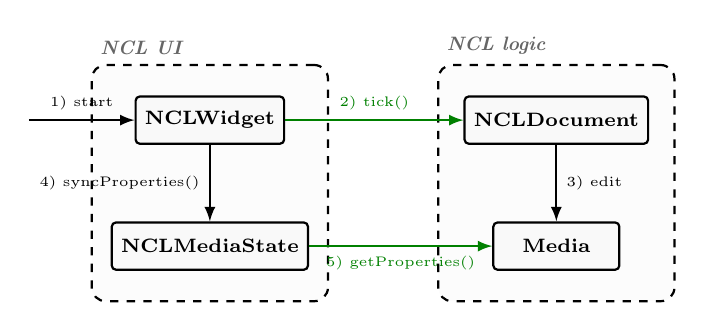
\begin{tikzpicture}[
    package/.style={draw, rectangle, rounded corners=5pt, minimum width=3.0cm, minimum height=3.0cm, fill=gray!2, dashed, thick, align=center},
    comp/.style={draw, rectangle, rounded corners=1.5pt, minimum width=1.6cm, minimum height=0.6cm, fill=gray!5, thick, align=center, font=\scriptsize},
    arrow/.style={-latex, thick},
    greenarrow/.style={-latex, thick, color=green!50!black}
  ]
    \node[package] (app_pkg) at (0, 0) {};
    \node[anchor=south west, font=\scriptsize\bfseries\itshape, text=gray!80!black] at (app_pkg.north west) {NCL UI};

    \node[comp] (ncl_widget) at (0, 0.8) {\textbf{NCLWidget}};
    \node[comp] (widgets) at (0, -0.8) {\textbf{NCLMediaState}};

    \node[package] (doc_pkg) at (4.4, 0) {};
    \node[anchor=south west, font=\scriptsize\bfseries\itshape, text=gray!80!black] at (doc_pkg.north west) {NCL logic};

    \node[comp] (ncl_doc_class) at (4.4, 0.8) {\textbf{NCLDocument}};
    \node[comp] (ncl_elements) at (4.4, -0.8) {\textbf{Media}};

    \draw[arrow] (-2.3, 0.8) -- (ncl_widget.west) node[midway, above, font=\tiny] {1) start};
    \draw[greenarrow] (ncl_widget) -- (ncl_doc_class) node[midway, above, font=\tiny] {2) tick()};
    \draw[arrow] (ncl_doc_class) -- (ncl_elements) node[midway, right, font=\tiny] {3) edit};
    \draw[arrow] (ncl_widget) -- (widgets) node[midway, left, font=\tiny] {4) syncProperties()};
    \draw[greenarrow] (widgets) -- (ncl_elements) node[midway, below, font=\tiny] {5) getProperties()};
  \end{tikzpicture}
  \Description{Communication diagram of gingaf showing the execution flow where the presentation components drive the document via ticks, and synchronize properties asynchronously without blocking the core execution logic.}
  \caption{\projectname{} communication diagram}
  \label{fig:arch}
\end{figure}

\subsection{\projectname{} NCL Logic}
\label{sec:ncllogic}

The \texttt{NCLDocument} class is the core of the NCL logic component. The execution state of \texttt{NCLDocument} is managed through three key API methods: \texttt{start()} to initialize execution; \texttt{tick()} to advance the virtual clock and process NCL logic; and \texttt{stop()} to halt execution.

The \texttt{start()} function begins by parsing the NCL XML input and validating the resulting tree against XSD rules, checking ID uniqueness and IDREF integrity. When the \texttt{start()} ends, \texttt{NCLDocument} will have the following data structures:
\begin{itemize}
  \item \texttt{DOM} (Document Object Model) contains \texttt{Element} instances in the document structure (Figure~\ref{fig:elem_tree}). Each \texttt{Element} contains its respective XML string and its raw XML attributes. \texttt{Node} extends \texttt{Element} to hold runtime state (sleeping, occurring, or paused) and a property list. \texttt{NCLua} is a special Media that executes Lua scripts in pure Dart\footnote{\url{https://pub.dev/packages/lua_dardo_plus}} for multiplatform (other elements were omitted for simplicity).
  \item \texttt{VirtualClock}: the engine maintains an internal logical clock which Media use for their elapsed time. This clock is advanced via \texttt{tick()} calls (ideal for debugging).
  \item \texttt{ActionQueue}: inside one \texttt{tick()}, actions are queued and drained deterministically to ensure consistent execution behavior.
  \item \texttt{UIQueue}: A shared queue that serves UI and logic without coupling them. At the end of tick, the Document writes entries indicating which \texttt{Media} nodes changed visual properties, so the UI component can update rendering accordingly. Moreover, before each tick, the NCL UI component can write entries to notify the document that a media presentation has ended (\textit{e.g.}, a video file reached its end), allowing the engine to process the corresponding event and propagate any triggered links.
\end{itemize}

\begin{figure}[ht]
  \centering
  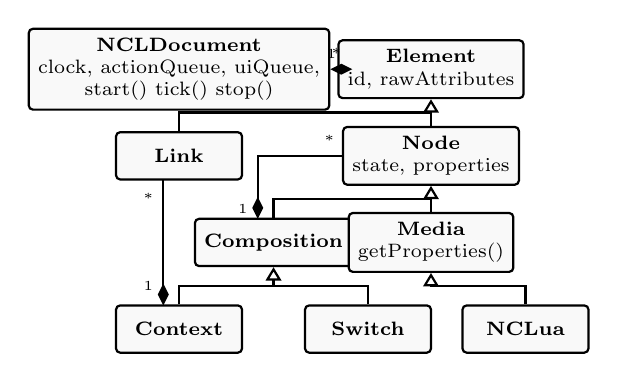
\begin{tikzpicture}[
    classbox/.style={draw, rectangle, rounded corners=1.5pt, minimum width=1.6cm, minimum height=0.6cm, align=center, fill=gray!5, thick, font=\scriptsize}
  ]
    \node [classbox] (ncldoc) at (-2.2, 2.0) {\textbf{NCLDocument} \\ clock, actionQueue, uiQueue, \\ start() tick() stop()};
    \node [classbox] (element) at (1.0, 2.0) {\textbf{Element} \\ id, rawAttributes};
    \node [classbox] (link) at (-2.2, 0.9) {\textbf{Link}};
    \node [classbox] (node) at (1.0, 0.9) {\textbf{Node} \\ state, properties};
    \node [classbox] (composition) at (-1.0, -0.2) {\textbf{Composition}};
    \node [classbox] (media) at (1.0, -0.2) {\textbf{Media} \\ getProperties()};
    \node [classbox] (context) at (-2.2, -1.3) {\textbf{Context}};
    \node [classbox] (switch) at (0.2, -1.3) {\textbf{Switch}};
    \node [classbox] (nclua) at (2.2, -1.3) {\textbf{NCLua}};

    \draw [thick, -{Triangle[open]}] (node.north) -- (element.south);
    \draw [thick] (link.north) |- (1.0, 1.45);
    
    \draw [thick, -{Triangle[open]}] (media.north) -- (node.south);
    \draw [thick] (composition.north) |- (1.0, 0.35);

    \draw [thick, -{Triangle[open]}] (context.north) |- (-1.0, -0.75) -- (composition.south);
    \draw [thick] (switch.north) |- (-1.0, -0.75);
    \draw [thick, -{Triangle[open]}] (nclua.north) |- (1.0, -0.75) -- (media.south);

    \draw [thick, {Diamond[fill=black]}-] (ncldoc.east) -- node[above, pos=0.15, font=\tiny] {1} node[above, pos=0.85, font=\tiny] {*} (element.west);
    \draw [thick, {Diamond[fill=black]}-] (-1.2, 0.1) -- node[left, pos=0.15, font=\tiny] {1} (-1.2, 0.9) -- node[above, pos=0.85, font=\tiny] {*} (node.west);
    \draw [thick, {Diamond[fill=black]}-] (-2.4, -1.0) -- node[left, pos=0.15, font=\tiny] {1} node[left, pos=0.85, font=\tiny] {*} (-2.4, 0.6);
  \end{tikzpicture}
  \Description{Class diagram showing the DOM representation of NCL elements in the gingaf logic package, highlighting NCLDocument, Element, Node, Media, Composition, and NCLua subclasses.}
  \caption{\texttt{gingaf} NCL \texttt{DOM}}
  \label{fig:elem_tree}
\end{figure}

\texttt{tick()} function advances an internal virtual clock by the given millisecond increment rather than relying on system time. This clock can be driven manually for testing or automatically by a Flutter periodic timer in a presentation environment. Decoupling time from the renderer enables high-speed headless testing: synchronization scenarios can be validated in-memory using inline XML strings, with no overhead from rendering windows, graphics libraries, or AV decoders.

On each call, \texttt{tick()} drains two queues. The \texttt{ActionQueue} collects transitions and link executions generated during state changes; these are drained deterministically in XML document definition order to ensure consistent execution behavior. The \texttt{UIQueue} serves communication across the component boundary: before the tick, the NCL UI component writes entries reporting that a media presentation has ended, which the engine processes to propagate any triggered links; after the tick, the engine writes entries indicating which \texttt{Media} nodes changed visual properties, so the NCL UI component can update rendering accordingly.

An example of the execution log produced during headless execution is shown in Listing~\ref{lst:logs}.

\begin{lstlisting}[caption={Headless execution log of video.ncl using \texttt{dart run ncl\_doc/lib/main.dart video.ncl}}, basicstyle=\scriptsize\ttfamily, frame=single, breaklines=true, aboveskip=1mm, belowskip=1mm, captionpos=b, numbers=left, label={lst:logs}]
> dart run ncl_doc/lib/main.dart examples/video.ncl
[ncl_doc_cli] Executing examples/video.ncl in headless mode
[Clock: 0.0s] NCLDocument will start
[Clock: 0.0s] Node "body": sleeping->occurring
[Clock: 0.0s] Node "video": sleeping->occurring
[ncl_doc_cli] perform 1 ticks per second indefinitely
[Clock: 0.0s] tickIndefinitely (1 ticks per/s)
[Clock: 1.0s] Tick
[Clock: 2.0s] Node "video" (area a1): sleeping->occurring
[Clock: 2.0s] Node "green_bg": sleeping->occurring
[Clock: 2.0s] Tick
[Clock: 3.0s] Tick
[Clock: 4.0s] Node "video" (area a1): occurring -> sleeping
[Clock: 4.0s] Node "green_bg": occurring -> sleeping
[Clock: 4.0s] Node "red_bg": sleeping->occurring
\end{lstlisting}

The reliability of the cross-platform codebase is maintained through an automated test suite. The \texttt{ncl\_doc} logic package contains 64 unit tests validating the parser and virtual clock progression. Because Dart compiles efficiently to JavaScript, all tests run in milliseconds directly in continuous integration pipelines on the web.

\subsection{\projectname{} NCL UI}
\label{sec:nclui2}

The \projectname{} NCL UI layer is responsible for visual presentation. \texttt{NCLWidget} drives the engine by calling \texttt{tick()} on \texttt{NCLDocument} (arrow~2 in Figure~\ref{fig:arch}) and delegates rendering to \texttt{NCLMediaState}, which reads the current visual properties of each \texttt{Media} node directly from the NCL logic component (arrow~5). The interface consists of a root \texttt{Ginga} widget that uses a Flutter \texttt{Stack} to lay out elements. A background audio/video widget (\texttt{main\_av\_widget}) is placed at the bottom, while the active media elements are rendered on top within the NCL presentation surface. The \texttt{WidgetFactory} maps NCL elements to native Flutter widgets. 

Currently implemented widgets include \texttt{ImageWidget} (which displays images and handles image format caching), \texttt{AVWidget} (which renders native video/audio playback and supports state tracking), and \texttt{TextWidget} (which renders formatted text blocks using bounds properties). Each widget extends \texttt{BaseWidget} to map NCL layout properties (such as \texttt{left}, \texttt{top}, \texttt{width}, \texttt{height}, and \texttt{background}) to Flutter's \texttt{Positioned} and \texttt{BoxDecoration} parameters.

A key design aspect of \projectname{} is the bidirectional event feedback loop. \texttt{NCLWidget} holds an instance of \texttt{NCLDocument} and registers a Flutter periodic timer that periodically calls \texttt{doc.tick()} to advance the virtual clock.

When a media widget experiences a state change (for example, when an \texttt{AVWidget} reaches the end of its video file), the widget notifies the \texttt{NCLWidget} via the UI Queue. The application then retrieves the corresponding \texttt{Media} node from the document and triggers its transition event, allowing the headless execution engine to run link conditions and propagate state changes back to the widgets. This ensures a clean separation of concerns: widgets only worry about rendering and local lifecycle events, while the engine handles the declarative NCL coordination logic.

To show the correctness and multiplatform execution capabilities of \projectname{}, we execute the sample NCL application (\texttt{video.ncl}) described in Section~\ref{sec:background}. As a result, Figure~\ref{fig:multiplatform} presents the execution of this application across three different environments: Windows, mobile (Android), and Web. Additionally, the temporal execution screenshots are shown in Figure~\ref{fig:multiplatform} and the corresponding headless simulation logs are provided in Listing~\ref{lst:logs} (Section~\ref{sec:ncllogic}).

\begin{figure}[ht]
  \centering
  \begin{subfigure}{0.7\linewidth}
    \centering
    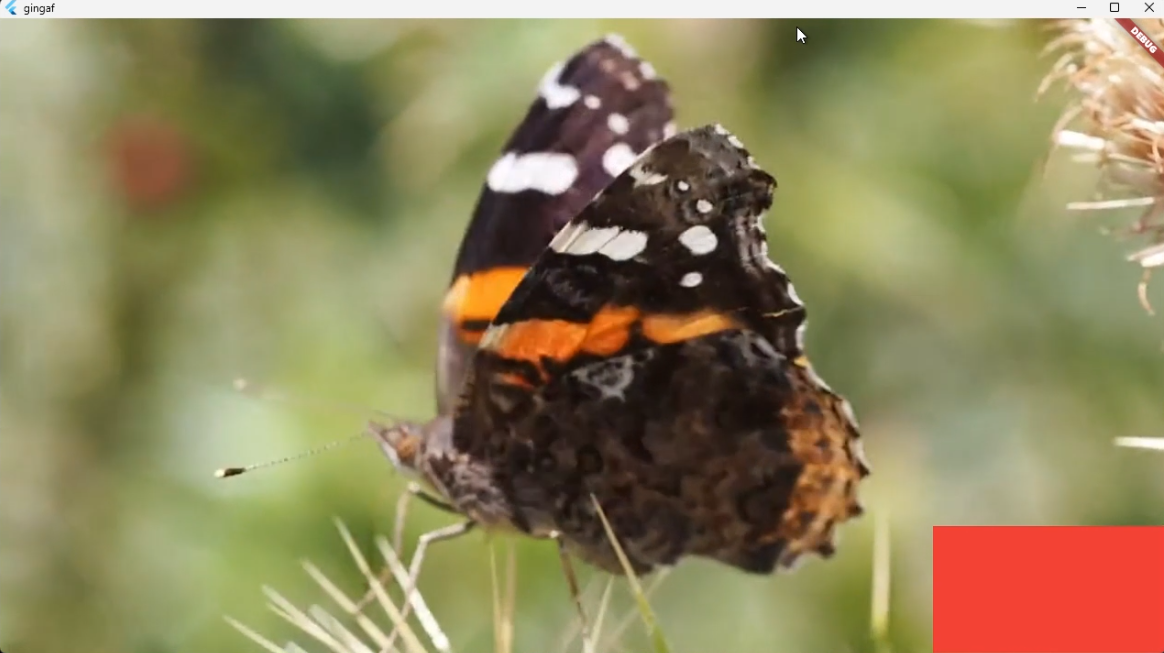
\includegraphics[width=\linewidth]{app_clock4.png}
    \Description{Sample NCL application execution on Windows showing a video player with a green overlay in the bottom-left.}
    \caption{Windows.}
    \label{fig:res_windows}
  \end{subfigure}%
  \hfill%
  \begin{subfigure}{0.3\linewidth}
    \centering
    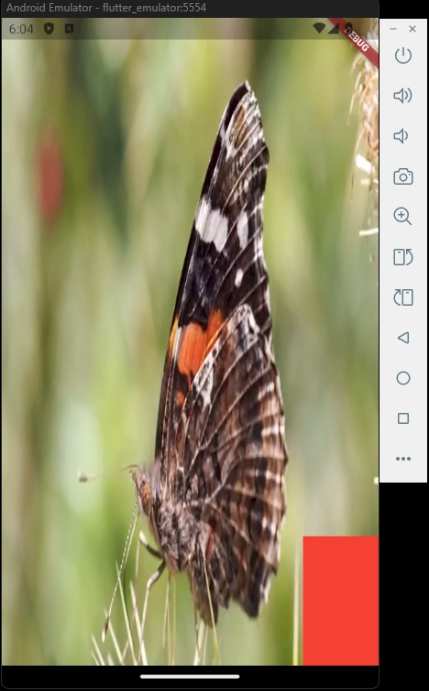
\includegraphics[height=3.4cm, keepaspectratio]{android.png}
    \Description{Sample NCL application execution on Android showing the video player with a green overlay.}
    \caption{Android.}
    \label{fig:res_android}
  \end{subfigure}%
  \begin{subfigure}{0.4\linewidth}
    \centering
    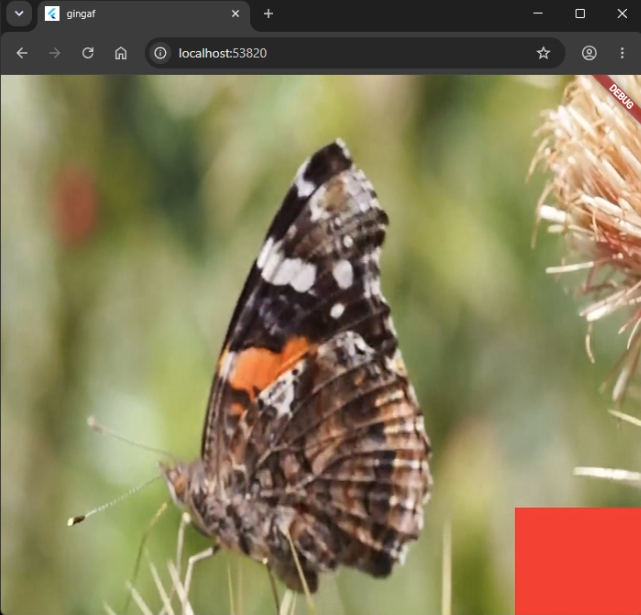
\includegraphics[width=\linewidth]{web.png}
    \Description{Sample NCL application execution on a Web browser showing the video player with a green overlay.}
    \caption{Web.}
    \label{fig:res_web}
  \end{subfigure}
  \caption{Multiplatform execution of \texttt{video.ncl} across Windows, Android, and Web.}
  \label{fig:multiplatform}
\end{figure}

The reliability of the codebase is maintained through an automated test suite. The \texttt{ncl\_doc} logic package contains 64 unit tests validating the parser, XML parsing rules, virtual clock progression, and deterministic link execution. The \texttt{gingaf} presentation package contains 14 tests verifying widget rendering, layout constraint resolution, focus state transitions, and integration with the NCL execution engine. All tests run in milliseconds due to the headless execution capabilities of the engine.

\subsection{\projectname{} NCLua}
\label{sec:nclua}

A key component of the Ginga architecture is NCLua, which enables the execution of imperative Lua scripts within the NCL document. Historically, implementing NCLua on the web has been an insurmountable challenge because it required linking the standard C Lua interpreter to the web environment, typically using complex Emscripten toolchains that are difficult to integrate transparently with the DOM and modern frameworks like Flutter.

To overcome this, \projectname{} adopts a novel approach: it implements the NCLua player entirely in Dart using the \texttt{lua\_dardo} library. \texttt{lua\_dardo} is a pure Dart implementation of the Lua 5.3 interpreter. Because it is written natively in Dart, it compiles directly to JavaScript and WebAssembly along with the rest of the \projectname{} logic, seamlessly running in any web browser without external C dependencies or WebAssembly bridges.

When an NCL document defines a Lua media element, \projectname{} instantiates a \texttt{lua\_dardo} state machine and binds the required NCLua APIs. These APIs allow the Lua script to register event listeners, query the NCL document properties, and emit events that the main \texttt{NCLDocument} logic can capture during its \texttt{tick()} cycle.

A major feature of NCLua is its ability to draw graphics onto a canvas using imperative commands. In a native C++ Ginga player, these commands call down into SDL or GTK canvas primitives. In a web environment, translating these calls synchronously across language barriers (\textit{e.g.}, JavaScript to Dart to C) is cumbersome. \projectname{} overcomes this by using a pure Dart Lua interpreter (\texttt{lua\_dardo}) to allow portability and a ``Command List'' abstraction. When the Lua script executes a drawing function (\textit{e.g.}, \texttt{canvas:drawLine()}) the Lua interpreter intercepts the call and appends a lightweight, serializable command object to an internal list. This list acts as an intermediate representation of the visual frame. At the end of the Lua script's execution slice, the NCL UI queries this list. The Flutter rendering engine then iterates over the list, translating each stored command directly into native Flutter \texttt{Canvas} operations (\textit{e.g.}, \texttt{canvas.drawLine()} or \texttt{canvas.drawParagraph()}). Figure~\ref{fig:lua_pipeline} illustrates this pipeline.

\begin{figure}[ht!]
  \centering
  \resizebox{\columnwidth}{!}{
  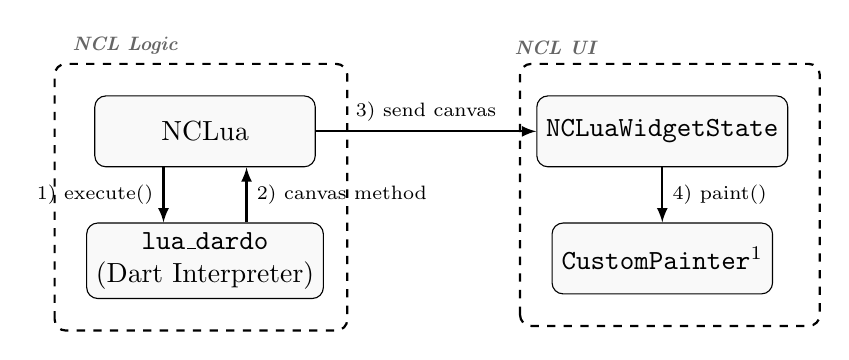
\begin{tikzpicture}[
    node distance=0.7cm and 2.8cm,
    block/.style={draw, rectangle, rounded corners, minimum width=2.8cm, minimum height=0.9cm, align=center, fill=gray!5},
    arrow/.style={-latex, thick},
    gingafbox/.style={draw, rectangle, rounded corners=4pt, dashed, thick, fill=none}
  ]
    \node[block] (nclua) {NCLua};
    \node[block, below=of nclua] (interpreter) {\texttt{lua\_dardo}\\(Dart Interpreter)};

    \node[block, right=2.8cm of nclua] (luawidget) {\texttt{NCLuaWidgetState}};
    \node[block, below=of luawidget] (painter) {\texttt{CustomPainter}\footnotemark};

    % Logic Box
    \draw[gingafbox] ($(interpreter.south west) + (-0.4,-0.4)$) rectangle ($(nclua.north east) + (0.4,0.4)$);
    \node[anchor=south west, font=\scriptsize\bfseries\itshape, text=gray!80!black] at ($(nclua.north west) + (-0.4,0.4)$) {NCL Logic};

    % UI Box
    \draw[gingafbox] ($(painter.south west) + (-0.4,-0.4)$) rectangle ($(luawidget.north east) + (0.4,0.4)$);
    \node[anchor=south west, font=\scriptsize\bfseries\itshape, text=gray!80!black] at ($(luawidget.north west) + (-0.4,0.4)$) {NCL UI};

    \draw[arrow] ([xshift=-15pt]nclua.south) -- node[left, font=\scriptsize] {1) execute()} ([xshift=-15pt]interpreter.north);
    \draw[arrow] ([xshift=15pt]interpreter.north) -- node[right, font=\scriptsize] {2) canvas method} ([xshift=15pt]nclua.south);
    \draw[arrow] (nclua.east) -- node[above, font=\scriptsize] {3) send canvas} (luawidget.west);
    \draw[arrow] (luawidget.south) -- node[right, font=\scriptsize] {4) paint()} (painter.north);
  \end{tikzpicture}
  }
  \Description{Pipeline diagram showing how Lua canvas drawing calls from lua_dardo are buffered in NCLua and sent as command lists to the CustomPainter in NCLuaWidgetState for rendering.}
  \caption{The NCLua Canvas Translation Pipeline. NCLua executes Lua via \texttt{lua\_dardo}, which calls back canvas methods. NCLua forwards those calls to \texttt{NCLuaWidgetState}, which delegates rendering to a \texttt{CustomPainter}.}
  \label{fig:lua_pipeline}
\end{figure}
\footnotetext{\url{https://api.flutter.dev/flutter/rendering/CustomPainter-class.html}}

This architecture offers two immense benefits for the web. First, the command list completely decouples the imperative execution speed of Lua from the browser's rendering framerate. Second, it maintains absolute cross-platform consistency, as Flutter guarantees identical canvas rendering semantics whether the application is running as a WebGL application, a Windows desktop app, or an iOS native application.

Handling asynchronous Lua operations, such as network requests or timers, within the Dart event loop requires careful synchronization. \projectname{} maps Lua's coroutine mechanisms to Dart's \texttt{Future} and \texttt{async/await} paradigms. When a Lua script invokes an asynchronous NCLua API, the \texttt{lua\_dardo} interpreter suspends execution and yields control back to the \texttt{NCLDocument}. Once the asynchronous operation completes, the engine resumes the Lua coroutine, passing the result back. This ensures that long-running Lua tasks do not block the main NCL execution thread, maintaining precise temporal synchronization across the entire document.

\section{Cross-Platform Ginga-HTML5 and Ginga-CC-WebServices}
\label{sec:htmlccws}

The Ginga standard specifies support for embedded HTML5 applications via Ginga-HTML5. In a traditional set-top box environment, this involves integrating an entire WebKit or Chromium instance into the C++ player, creating a massive platform dependency that requires complex cross-platform configuration. \projectname{} reduces this complexity by implementing Ginga-HTML5 using the Dart \texttt{webview\_all} package\footnote{\url{https://pub.dev/packages/webview_all}}. This package abstracts the respective web engines on mobile (\textit{e.g.}, Android WebView\footnote{\url{https://developer.android.com/reference/android/webkit/WebView}}) and desktop (OS-specific webviews, \textit{e.g.}, WebView2\footnote{\url{https://developer.microsoft.com/microsoft-edge/webview2}}), while using JavaScript interoperability on the web. Moreover, a critical aspect of Ginga-HTML5 is its integration with CCWS, which defines REST APIs that allow the HTML application to access Ginga-CC capabilities, control the main video, and interact with the broadcast stream.

When running natively on desktop or mobile environments (Figure~\ref{fig:ccws_intercept}a), \projectname{} executes Ginga-HTML5 applications within a native WebView container. To support CCWS, the architecture embeds a local \texttt{HTTPServer} listening by default on port 44642. The HTML application makes standard HTTP requests targeting this local server, which handles routing, processes requests against the NCL document context, and returns standard HTTP responses.

When running in a web browser environment (Figure~\ref{fig:ccws_intercept}b), executing a local HTTP server is not possible due to browser security restrictions and sandbox limitations. To bypass this, \projectname{} executes the HTML application in a sandboxed \texttt{iframe} and virtualizes the CCWS middleware without an HTTP server. This is achieved by injecting a lightweight JavaScript shim into the \texttt{iframe} that overloads the standard browser \texttt{fetch} API and \texttt{XMLHttpRequest} objects. When the HTML application makes a request targeting a CCWS endpoint, the overloaded \texttt{fetch} intercepts it and dispatches a cross-origin message (\texttt{postMessage}) to the parent Dart/Flutter application. The parent application receives this message, routes it internally to the CCWS logic manager, and returns the response payload back to the iframe. The overloaded \texttt{fetch} then resolves its Promise with this mock response, completely transparent to the HTML application. This architecture successfully virtualizes the CCWS middleware entirely within the browser, eliminating the need for any backend or local HTTP server.

\begin{figure}[ht!]
  \centering
  \begin{subfigure}{0.48\linewidth}
    \centering
    \resizebox{\columnwidth}{!}{
    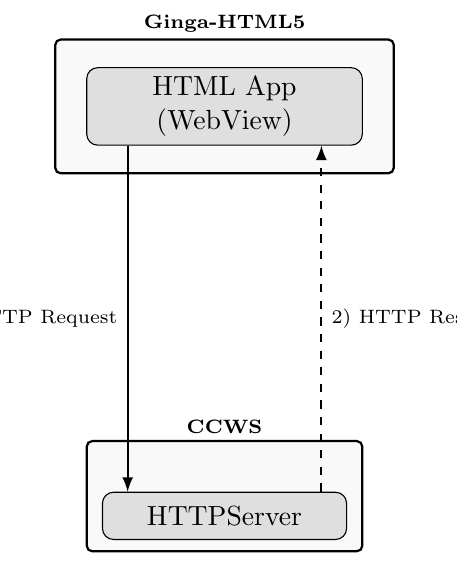
\begin{tikzpicture}[
      node distance=0.4cm and 0cm,
      block/.style={draw, rectangle, rounded corners, minimum width=3.5cm, minimum height=0.9cm, align=center, fill=gray!25},
      outerbox/.style={draw, rectangle, rounded corners=2pt, thick, minimum width=3.5cm, minimum height=1.4cm, fill=gray!5},
      innerbox/.style={draw, rectangle, rounded corners, minimum width=3.1cm, minimum height=0.6cm, align=center, fill=gray!25},
      arrow/.style={-latex, thick},
      gingafbox/.style={draw, rectangle, rounded corners=4pt, dashed, thick, fill=none}
    ]
      \useasboundingbox (-2.5, -5.7) rectangle (2.6, 1.0);
      \node[outerbox, minimum width=4.3cm, minimum height=1.7cm] (html5_outer) at (0, 0) {};
      \node[anchor=south, font=\scriptsize\bfseries, inner sep=2pt] at (html5_outer.north) {Ginga-HTML5};
      
      \node[block] (htmlapp) {HTML App\\(WebView)};
      \node[block, below=of htmlapp, draw=none, fill=none, text opacity=0] (shim) {Fetch Overload\\Shim};
      \node[block, below=of shim, draw=none, fill=none, text opacity=0] (flutter) {Flutter NCL UI};
      
      \node[outerbox] (ccws) at (0, -4.95) {};
      \node[anchor=south, font=\scriptsize\bfseries, inner sep=2pt] at (ccws.north) {\CCWS};
      \node[innerbox] (httpserver) at (0, -5.2) {HTTPServer};
      
      \draw[arrow] ([xshift=-35pt]htmlapp.south) -- node[left, font=\scriptsize] {1) HTTP Request} ([xshift=-35pt]httpserver.north);
      \draw[arrow, dashed] ([xshift=35pt]httpserver.north) -- node[right, font=\scriptsize] {2) HTTP Response} ([xshift=35pt]htmlapp.south);
    \end{tikzpicture}
    }
    \caption{Native Clients}
  \end{subfigure}%
  \hfill%
  \begin{subfigure}{0.48\linewidth}
    \centering
    \resizebox{\columnwidth}{!}{
    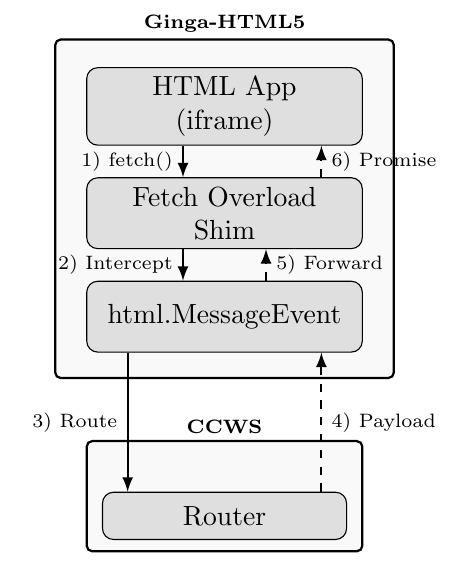
\begin{tikzpicture}[
      node distance=0.4cm and 0cm,
      block/.style={draw, rectangle, rounded corners, minimum width=3.5cm, minimum height=0.9cm, align=center, fill=gray!25},
      outerbox/.style={draw, rectangle, rounded corners=2pt, thick, minimum width=3.5cm, minimum height=1.4cm, fill=gray!5},
      innerbox/.style={draw, rectangle, rounded corners, minimum width=3.1cm, minimum height=0.6cm, align=center, fill=gray!25},
      arrow/.style={-latex, thick},
      gingafbox/.style={draw, rectangle, rounded corners=4pt, dashed, thick, fill=none}
    ]
      \useasboundingbox (-2.5, -5.7) rectangle (2.6, 1.0);
      \node[outerbox, minimum width=4.3cm, minimum height=4.3cm] (html5_outer) at (0, -1.3) {};
      \node[anchor=south, font=\scriptsize\bfseries, inner sep=2pt] at (html5_outer.north) {Ginga-HTML5};
      
      \node[block] (htmlapp) {HTML App\\(iframe)};
      \node[block, below=of htmlapp] (shim) {Fetch Overload\\Shim};
      \node[block, below=of shim] (flutter) {html.MessageEvent};
      
      \node[outerbox] (ccws) at (0, -4.95) {};
      \node[anchor=south, font=\scriptsize\bfseries, inner sep=2pt] at (ccws.north) {\CCWS};
      \node[innerbox] (router) at (0, -5.2) {Router};
      
      \draw[arrow] ([xshift=-15pt]htmlapp.south) -- node[left, font=\scriptsize] {1) fetch()} ([xshift=-15pt]shim.north);
      \draw[arrow] ([xshift=-15pt]shim.south) -- node[left, font=\scriptsize] {2) Intercept} ([xshift=-15pt]flutter.north);
      \draw[arrow] ([xshift=-35pt]flutter.south) -- node[left, font=\scriptsize] {3) Route} ([xshift=-35pt]router.north);
      \draw[arrow, dashed] ([xshift=35pt]router.north) -- node[right, font=\scriptsize] {4) Payload} ([xshift=35pt]flutter.south);
      \draw[arrow, dashed] ([xshift=15pt]flutter.north) -- node[right, font=\scriptsize] {5) Forward} ([xshift=15pt]shim.south);
      \draw[arrow, dashed] ([xshift=35pt]shim.north) -- node[right, font=\scriptsize] {6) Promise} ([xshift=35pt]htmlapp.south);
    \end{tikzpicture}
    }
    \caption{Web Client}
  \end{subfigure}
  \Description{Diagram of the CCWS request Architecture, comparing the HTTP Request/Response flow on Native Clients with the fetch overloading shim mechanism on the Web Client.}
  \caption{CCWS Request Architecture across different platforms. Native clients bridge WebView requests directly, while the Web client overloads \texttt{fetch} in a sandboxed iframe using \texttt{postMessage}.}
  \label{fig:ccws_intercept}
\end{figure}

\section{Use case: GingaPlayground}
\label{sec:playground}
To validate our proposed decoupled architecture and verify that the core logic engine can run deterministically in a pure web sandbox, we developed GingaPlayground. This web-based editor use case serves to confirm the feasibility of our decoupled approach by integrating the Flutter UI for rendering the application, a code editor\footnote{\url{https://microsoft.github.io/monaco-editor/}} for modifying NCL and Lua source files in real-time, and the cross-platform NCL logic running entirely in the browser.

This implementation directly validates that separating the NCL state from the UI renderer allows the logic engine to compile to JavaScript and Wasm, enabling instant, configuration-free execution without native desktop bindings or local virtualization. Through this environment, developers can visually inspect document states, manipulate the execution timeline, and dynamically reload modifications without leaving the browser, confirming that our solution provides similar execution capabilities compared to traditional players.

Figure~\ref{fig:playground_res} presents the visual execution of the sample Ginga-NCL application (\texttt{video.ncl}) from Listing~\ref{lst:ncl}, the Ginga-HTML5 application from Listing~\ref{lst:html5}, and a NCLua application with canvas calls(\texttt{lua\_canvas.ncl}) directly inside Google Chrome without any native plugins. The figure demonstrates the GingaPlayground interface layout, where the left side serves as the web-based code editor and the right side displays the real-time execution of the running Ginga application. This proves that both the temporal synchronization defined in the NCL links and the imperative NCLua drawing commands are rendered correctly in the browser.

\section{Final Remarks}
\label{sec:remarks}


\projectname{} demonstrates that decoupling the Ginga logic and UI components provides a highly portable solution that successfully brings the Ginga middleware to cross-platform environments, including the web. By isolating the NCL state machine and execution engine in pure Dart, the logic runs fully in-memory and can compile directly to JavaScript or native binaries without platform-dependent bindings or multimedia pipeline dependencies. This separation of concerns allows developers to execute and test synchronization logic deterministically on any platform, while rendering is handled independently by the presentation layer. Our architecture resolves the historical portability challenges of traditional Ginga middleware by removing the tight coupling between execution logic and native rendering APIs.

Furthermore, this web-native architecture opens new possibilities for collaborative development and continuous integration of digital TV applications. Since the \projectname{} engine runs deterministically in the browser, NCL projects can be easily shared via URL links, embedded in documentation, or integrated into online tutorials. This portability not only benefits educational initiatives but also accelerates industrial prototyping. Broadcasters and application designers can quickly iterate on UI layouts, Lua scripting logic, and CCWS interactions without deploying the code to physical set-top boxes during the early stages of development, ultimately reducing the time-to-market for new interactive services.

The immediate next step in this research is to evolve the GingaPlayground by implementing a Language Server Protocol (LSP)\footnote{\url{https://microsoft.github.io/language-server-protocol/}} server. Integrating an LSP server is highly beneficial because it decouples the editor client (\textit{e.g.}, Monaco Editor or VS Code) from the core NCL validation and analysis engine. By encapsulating our Dart-based parser into a language server, we can deliver a consistent and feature-rich authoring experience, like real-time error reporting (diagnostics), context-aware autocompletion of NCL tags and attributes, and symbol outline navigation. Additionally, future work includes implementing support to allow Remote Players, for instance NCL360 formats~\cite{souza2020ncl360}.

\bibliographystyle{ACM-Reference-Format}
\bibliography{references}

\end{document}
